%%%%%%%%%%%%%%%%%%%%%%%%%%%%%%%%%%%%%%%%%%%%%%
% To select a journal, use its code for the 
% journal= option in the \documentclass command.
% The journal codes for this template are:

% Wearable Technologies: wet
% Data and Policy: dap
% Data-centric Engineering: dce
% Environmental Data Science: eds
% Programmable Materials: prm
% Journal of Nonlinear Waves: jnw
% Flow: flw
% Judgment and Decision Making: jdm
% Psychometrika: psy
% Forum of Mathematics, Pi: fmp
% Forum of Mathematics, Sigma: fms
% Glasgow Mathematical Journal: gmj
% Research Synthesis Methods: rsm
%%%%%%%%%%%%%%%%%%%%%%%%%%%%%%%%%%%%%%%%%%%%%%
\documentclass[journal=eds]{CAM-MODERN}%

% If using any of the following journal options:
%   wet, dap, dce, eds, prm, jnw, flw, jdm, psy, rsm
% then uncomment the following line:
\addbibresource{bibliography_zotero.bib}


%%%% Packages
\usepackage{graphicx}
\usepackage{multicol,multirow}
\usepackage{amsmath,amssymb,amsfonts}
\usepackage{mathrsfs}
\usepackage{amsthm}
\usepackage{rotating}
\usepackage{appendix}
\usepackage{ifpdf}
\usepackage[T1]{fontenc}
\usepackage{newtxtext}
% \usepackage{newtxmath}
\usepackage{textcomp}
\usepackage{xcolor}
\usepackage{lipsum}
\usepackage[colorlinks,allcolors=blue]{hyperref}
\usepackage{lineno}
\usepackage{subcaption}
\usepackage{lscape}
\usepackage{enumitem}
\usepackage{makecell}
\usepackage{microtype}
\usepackage{floatrow}
\usepackage{verbatim}
\usepackage{algorithm}
\usepackage{algpseudocode}

\newtheorem{theorem}{Theorem}[section]
\newtheorem{lemma}[theorem]{Lemma}
\theoremstyle{definition}
\newtheorem{remark}[theorem]{Remark}
\newtheorem{example}[theorem]{Example}
\numberwithin{equation}{section}

\jname{Environmental Data Science}
\articletype{PREPRINT}
%\artid{20}
\jyear{2025}
%\jvol{4}
%\jissue{1}
\raggedbottom

\graphicspath{{figures/}}

\newcommand{\detailtexcount}[1]{%
  \immediate\write18{texcount -merge -sum -q #1.tex > #1.wcdetail }%
  \verbatiminput{#1.wcdetail}%
}

% titlebox
\usepackage{tikzpagenodes,eso-pic,graphicx,xcolor}
\definecolor{cambridgeblue}{HTML}{A3C1AD}

\newlength\CoverSidePad     \setlength\CoverSidePad{2.5\parindent}       % left/right padding
\newlength\CoverTopPad      \setlength\CoverTopPad{1.75\baselineskip}       % top padding
\newlength\CoverBottomLift  \setlength\CoverBottomLift{.175\textheight}  % how far above bottom to stop


% Rounded Cambridge-blue card behind page 1
\AddToHook{shipout/background}{%
  \ifnum\value{page}=1\relax
  \begin{tikzpicture}[remember picture,overlay]
    % insets from paper edge so it surrounds the header logo too
    \def\Inset{8mm}
    \def\BottomLift{30mm}
    \path (current page.north west) ++(\CoverSidePad,-\CoverTopPad) coordinate (NW);
    \path (current page.south east) ++(-\CoverSidePad,\CoverBottomLift) coordinate (SE);
    \filldraw[rounded corners=8pt,
              fill=cambridgeblue!12,
              draw=none,
              line width=0.8pt] (NW) rectangle (SE);
  \end{tikzpicture}%
  \fi
}


\begin{document}


%TC:ignore
\begin{Frontmatter}

\title[Short Title]{Title goes here}

\author[1]{Author One}
\author[2]{Author Two}
\authormark{Author One et al.}

\address[1]{Department, University, Country}
\address[2]{Department, University, Country}

\keywords{keyword1, keyword2, keyword3}

\abstract{
Abstracts should be 250 words. It must be able to stand alone and so cannot contain citations to the paper's references, equations, etc. An abstract must consist of a single paragraph and be concise. Because of online formatting, abstracts must appear as plain as possible.
}

\plainsummary{
A plain language summary should be written in accessible terms for non-specialist readers. It is typically 150–200 words and explains the purpose of the study, the approach used, and the key findings without technical jargon, equations, or references. The summary should be clear, concise, and free of abbreviations or specialised terminology so that it can be understood by the general public, policymakers, and researchers in other disciplines.
}

\end{Frontmatter}
%TC:endignore

\clearpage
\linenumbers

\section{Insert A head here}
This demo file is intended to serve as a ``starter file''. It is for preparing manuscript submission only, not for preparing camera-ready versions of manuscripts. Manuscripts will be typeset for publication by the journal, after they have been accepted.

By default, this template uses \texttt{bibtex} and adopts the AMS referencing style. However, the journal you’re submitting to may require a different reference style; specify the journal you're using with the class' \texttt{journal} option --- see lines 1--19 of \emph{Sample.tex} for a list of options and instructions for selecting the journal. 

Overleaf will run \texttt{pdflatex} and \texttt{bibtex} automatically as needed. But if you had \emph{first} compiled using another \texttt{journal} option that adopts \texttt{biblatex}, and \emph{then} change the \texttt{journal} option to one that adopts Bib\TeX{}, you may get some compile error messages instead. In this case you will need to do a `Recompile from scratch'; see \url{https://www.overleaf.com/learn/how-to/Clearing_the_cache}.

On a local \LaTeX{} installation, you would need to run these steps instead:
\begin{enumerate}
    \item Delete \texttt{sample.aux}, \texttt{sample.bbl} if these files from a previous compile using \texttt{biber} still exist.
    \item \verb|pdflatex sample|
    \item \verb|bibtex sample|
    \item \verb|pdflatex sample|
    \item \verb|pdflatex sample|
\end{enumerate}

Some journals e.g.~\texttt{journal=wet} require \texttt{biblatex}. For such journals, you will need to
\begin{itemize}
    \item uncomment the existing \verb|\addbibresource{example.bib}|;
    \item change the existing \verb|\bibliography{example}| to be\\
    \verb|\printbibliography| instead.
\end{itemize} 

If you are submitting to a journal that uses \texttt{biblatex} and using this template on Overleaf, Overleaf's build tool will automatically run \texttt{pdflatex} and \texttt{biber}. If you are compiling this template on your own local \LaTeX{} installation, please execute the following commands:
\begin{enumerate}
    \item \verb|pdflatex sample|
    \item \verb|biber sample|
    \item \verb|pdflatex sample|
    \item \verb|pdflatex sample|
\end{enumerate}

\subsection{Insert B head here}

\lipsum[2]

\subsubsection{Insert C head here}

\lipsum[3]

\paragraph{Insert D head here}

\lipsum[4]

\section{Insert A head here}
\subsection{Insert B head here}
\subsubsection{Insert C head here}
\lipsum[4]\footnote{This is sample for footnote this is sample for footnote this is sample for footnote  this is sample for footnote this is sample for footnote.}

\section{Equations}

Equations in \LaTeX{} can either be inline or on-a-line by itself. For
inline equations use the \verb+$...$+ commands. Eg: The equation
$H\psi = E \psi$ is written via the command $H \psi = E \psi$.

For on-a-line by itself equations (with auto generated equation numbers)
one can use the equation or eqnarray environments \textit{D}.
\begin{equation}
\mathcal{L} = i {\psi} \gamma^\mu D_\mu \psi
    - \frac{1}{4} F_{\mu\nu}^a F^{a\mu\nu} - m {\psi} \psi
\label{eq1}
\end{equation}
where,
\begin{align}
D_\mu &=  \partial_\mu - ig \frac{\lambda^a}{2} A^a_\mu
\nonumber \\
F^a_{\mu\nu} &= \partial_\mu A^a_\nu - \partial_\nu A^a_\mu
    + g f^{abc} A^b_\mu A^a_\nu
\label{eq2}
\end{align}
Notice the use of \verb+\nonumber+ in the align environment at the end
of each line, except the last, so as not to produce equation numbers on
lines where no equation numbers are required. The \verb+\label{}+ command
should only be used at the last line of an align environment where
\verb+\nonumber+ is not used.
\begin{equation}
Y_\infty = \left( \frac{m}{\textrm{GeV}} \right)^{-3}
    \left[ 1 + \frac{3 \ln(m/\textrm{GeV})}{15}
    + \frac{\ln(c_2/5)}{15} \right]
\end{equation}
The class file also supports the use of \verb+\mathbb{}+, \verb+\mathscr{}+ and
\verb+\mathcal{}+ commands. As such \verb+\mathbb{R}+, \verb+\mathscr{R}+
and \verb+\mathcal{R}+ produces $\mathbb{R}$, $\mathscr{R}$ and $\mathcal{R}$
respectively.

\section{Figures}

As per the \LaTeX\ standards eps images in \verb!latex! and pdf/jpg/png images in
\verb!pdflatex! should be used. This is one of the major differences between \verb!latex!
and \verb!pdflatex!. The images should be single page documents. The command for inserting images
for latex and pdflatex can be generalized. The package that should be used
is the graphicx package.

\begin{figure}[t]%
\FIG{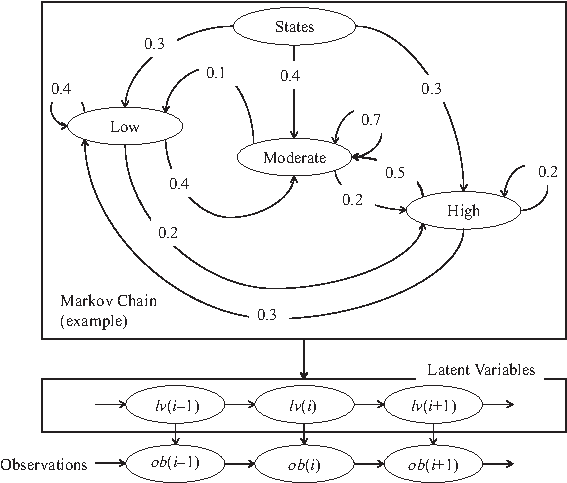
\includegraphics[width=0.9\textwidth]{placeholder-figure}}
{\caption{This is a widefig. This is an example of long caption this is an example of long caption  this is an example of long caption this is an example of long caption}
\label{fig1}}
\end{figure}



\section{Tables}

Tables can be inserted via the normal table and tabular environment. To put
footnotes inside tables one has to use the additional ``fntable" environment
enclosing the tabular environment. The footnote appears just below the table
itself.

\begin{table}[t]
\tabcolsep=0pt%
\TBL{\caption{Tables which are too long to fit,
should be written using the ``table*'' environment as~shown~here\label{tab2}}}
{\begin{fntable}
\begin{tabular*}{\textwidth}{@{\extracolsep{\fill}}lcccccc@{}}\toprule%
 & \multicolumn{3}{@{}c@{}}{\TCH{Element 1}}& \multicolumn{3}{@{}c@{}}{\TCH{Element 2\smash{\footnotemark[1]}}}
 \\\cmidrule{2-4}\cmidrule{5-7}%
\TCH{Projectile} & \TCH{Energy} & \TCH{$\sigma_{\mathit{calc}}$} & \TCH{$\sigma_{\mathit{expt}}$} &
\TCH{Energy} & \TCH{$\sigma_{\mathit{calc}}$} & \TCH{$\sigma_{\mathit{expt}}$} \\\midrule
\TCH{Element 3}&990 A &1168 &$1547\pm12$ &780 A &1166 &$1239\pm100$\\
{\TCH{Element 4}}&500 A &961 &$\hphantom{0}922\pm10$ &900 A &1268 &$1092\pm40\hphantom{0}$\\
\botrule
\end{tabular*}%
\footnotetext[]{{Note:} This is an example of table footnote this is an example of table footnote this is an example of table footnote this is an example of~table footnote this is an example of table footnote}
\footnotetext[1]{This is an example of table footnote}%
\end{fntable}}
\end{table}



\section{Cross referencing}

Environments such as figure, table, equation, align can have a label
declared via the \verb+\label{#label}+ command. For figures and table
environments one should use the \verb+\label{}+ command inside or just
below the \verb+\caption{}+ command.  One can then use the
\verb+\ref{#label}+ command to cross-reference them. As an example, consider
the label declared for Figure \ref{fig1} which is
\verb+\label{fig1}+. To cross-reference it, use the command
\verb+ Figure \ref{fig1}+, for which it comes up as
``Figure \ref{fig1}''.
The reference citations should used as per the ``natbib'' packages. Some sample citations:  \citep{sellers_global_1969}.

\section{Lists}

List in \LaTeX{} can be of three types: enumerate, itemize and description.
In each environments, new entry is added via the \verb+\item+ command.
Enumerate creates numbered lists, itemize creates bulleted lists and
description creates description lists.
\begin{enumerate}
\item First item in the number list.
\item Second item in the number list.
\item Third item in the number list.
\end{enumerate}
List in \LaTeX{} can be of three types: enumerate, itemize and description.
In each environments, new entry is added via the \verb+\item+ command.
\begin{itemize}
\item First item in the bullet list.
\item Second item in the bullet list.
\item Third item in the bullet list.
\end{itemize}

\begin{appendix}
\section{Appendix. Title for Appendix Section}\label{appendixA}
Appendix text here.
\end{appendix}


\section{Conclusion}

Some Conclusions here.



\begin{Backmatter}



\paragraph{Acknowledgments}
We are grateful for the technical assistance of A. Author.

\paragraph{Funding Statement}
This research was supported by grants from the <funder-name><doi>(<award ID>); <funder-name><doi>(<award ID>).

\paragraph{Competing Interests}
A statement about any financial, professional, contractual or personal relationships or situations that could be perceived to impact the presentation of the work --- or `None' if none exist

\paragraph{Code and Data Availability Statement}
A statement about how to access data, code and other materials allowing users to understand, verify and replicate findings --- e.g. Replication data and code can be found in Harvard Dataverse: \verb+\url{https://doi.org/link}+. %
% IMPORTANT
This manuscript was prepared using \LaTeX~(\url{https://www.latex-project.org}) on Overleaf~(\url{https://www.overleaf.com}) with the \texttt{cam-modern} template~(\url{https://github.com/p3jitnath/cam-modern}), derived from the Cambridge University Press \texttt{CUP-JNL-DTM} class (\url{https://www.overleaf.com/latex/templates/cup-data-template/kwrskzvmfxbq}).

\paragraph{Ethical Standards}
The research meets all ethical guidelines, including adherence to the legal requirements of the study country.

\paragraph{LLM Usage}
A statement about LLM Usage --- e.g. The authors acknowledge the use of AI language models, specifically ChatGPT~(GPT-5 Thinking mini and GPT-4o \url{https://chatgpt.com}), during the preparation of this work. These tools were used to polish language usage and improve the overall clarity of the manuscript, as well as to assist with designing plotting code for the graphs. All AI-generated content was reviewed, verified, and edited by the authors to ensure accuracy and appropriateness.

\paragraph{Author Contributions}
Please provide an author contributions statement using the CRediT taxonomy roles as a guide {\verb+\url{https://www.casrai.org/credit.html}+}. Conceptualization: A.A; A.B. Methodology: A.A; A.B. Data curation: A.C. Data visualisation: A.C. Writing original draft: A.A; A.B. All authors approved the final submitted draft.

\printbibliography

\end{Backmatter}

\end{document}